%%%%%%%%%% !TEX program = xelatex %%%%%%%%%%
% !TEX program = xelatex
\documentclass[a4paper,12pt,openany,twoside]{book}
% \documentclass[a4paper,12pt,openany,twoside]{ctexart}
% 当目录多于1页时，使用\thispagestyle{empty}和\pagestyle{empty}，都无法完全清除目录的页眉页脚格式，需要使用到下面的\AtBeginDocument{}代码
\AtBeginDocument{
	\addtocontents{toc}{\protect\thispagestyle{empty}}%
	\addtocontents{lof}{\protect\thispagestyle{empty}}%
}

\usepackage{caption}

% \usepackage{xcolor}
% \usepackage{soulutf8}
% \usepackage{array}
\input{setup/package}                      % 定义本文所使用宏包
\graphicspath{{figures/}}                  % 定义所有的.eps文件在figures子目录下
\setmainfont{Times New Roman}         %%%%%%%%%% 设置主英文字体
\begin{document}                           % 开始全文
% !Mode:: "TeX:UTF-8"
%  Authors: 杜佳宜      湖南大学

% Modified by Kim 深圳大学, 2023/03/04

%%%%%%%%%% 字体命令定义 %%%%%%%%%%%%%%%%%
% \setCJKfamilyfont{song}[Path=fonts/]{simsun.ttc}  % 设置宋体，指定字体路径
\setCJKfamilyfont{fs}[Path=fonts/]{simfang.ttf}  % 设置仿宋字体，指定字体路径
\setCJKfamilyfont{hei}[AutoFakeBold,Path=fonts/]{simhei.ttf}  % 设置黑体字体，指定字体路径
\newfontfamily\westernhei[Path=fonts/]{simhei.ttf}  % 西文也使用SimHei


\newcommand{\song}{\CJKfamily{song}}    % 宋体
\newcommand{\fs}{\CJKfamily{fs}}        % 仿宋体
\newcommand{\kai}{\CJKfamily{kai}}      % 楷体
% \newcommand{\hei}{\CJKfamily{hei}}      % 黑体
\newcommand{\hei}{\CJKfamily{hei}\westernhei}
\newcommand{\li}{\CJKfamily{li}}        % 隶书

\newcommand{\tnewroman}{\fontspec{Times New Roman}}
\newcommand{\adobegothicstdb}{\fontspec{Adobe Gothic Std B}}
\newcommand{\Centaur}{\fontspec{Centaur}}
\newcommand{\Lucida}{\fontspec[Path=fonts/,]{lucon.ttf}}    % 使用自定义字体
\newcommand{\simhei}{\fontspec[Path=fonts/,]{simhei.ttf}}    % 使用自定义字体
\newcommand{\Arial}{\fontspec[Path=fonts/,]{Arialbd.ttf}} %设置自定义字体



\newcommand{\yihao}{\fontsize{26pt}{26pt}\selectfont}       % 一号, 1.倍行距
\newcommand{\xiaoyi}{\fontsize{24pt}{24pt}\selectfont}      % 小一, 1.倍行距
\newcommand{\erhao}{\fontsize{22pt}{22pt}\selectfont}       % 二号, 1.倍行距
\newcommand{\xiaoer}{\fontsize{18pt}{18pt}\selectfont}      % 小二, 单倍行距
\newcommand{\sanhao}{\fontsize{16pt}{16pt}\selectfont}      % 三号, 1.倍行距
\newcommand{\xiaosan}{\fontsize{15pt}{15pt}\selectfont}     % 小三, 1.倍行距
\newcommand{\sihao}{\fontsize{14pt}{14pt}\selectfont}       % 四号, 1.0倍行距
\newcommand{\xiaosi}{\fontsize{12pt}{20pt}\selectfont}  	% 小四, 23磅行距
\newcommand{\wuhao}{\fontsize{10.5pt}{10.5pt}\selectfont}   % 五号, 单倍行距
\newcommand{\xiaowu}{\fontsize{9pt}{9pt}\selectfont}        % 小五, 单倍行距
\setlength{\headheight}{20pt}
%\CJKcaption{gb_452}
% \CJKtilde  % 重新定义了波浪符~的意义
\newcommand\prechaptername{第}
\newcommand\postchaptername{章}



% \xeCJKsetup{AutoFakeBold=true}
% \xeCJKsetup{AutoFakeBold=2.5}

% 调整罗列环境的布局 % Modified by Kim
\setitemize{leftmargin=0em,itemindent=3em,itemsep=0em,partopsep=0em,parsep=0em,topsep=-0em}
\setenumerate{leftmargin=0em,itemindent=3em,itemsep=0em,partopsep=0em,parsep=0em,topsep=0em}


%避免宏包 hyperref 和 arydshln 不兼容带来的目录链接失效的问题。
\def\temp{\relax}
\let\temp\addcontentsline
\gdef\addcontentsline{\phantomsection\temp}


% 自定义项目列表标签及格式 \begin{publist} 列表项 \end{publist}
\newcounter{pubctr} % 自定义新计数器
\newenvironment{publist}{%%%%% 定义新环境
\begin{list}{[\arabic{pubctr}]} %% 标签格式
    {
     \usecounter{pubctr}
     \setlength{\leftmargin}{2em}     % 左边界 \leftmargin =\itemindent + \labelwidth + \labelsep
     \setlength{\itemindent}{0em}     % 标号缩进量
     \setlength{\labelsep}{1em}       % 标号和列表项之间的距离,默认0.5em
     \setlength{\rightmargin}{0em}    % 右边界
     \setlength{\topsep}{0ex}         % 列表到上下文的垂直距离
     \setlength{\parsep}{0ex}         % 段落间距
     \setlength{\itemsep}{0ex}        % 标签间距
     \setlength{\listparindent}{0pt} % 段落缩进量
    }}
{\end{list}}%%%%%


\makeatletter
\renewcommand\normalsize{
  \@setfontsize\normalsize{12pt}{23pt} 	% 此处用于设置正文字体，小四号字体宋体（Times New Roman）
  \setlength\abovedisplayskip{4pt}
  \setlength\abovedisplayshortskip{4pt}
  \setlength\belowdisplayskip{\abovedisplayskip}
  \setlength\belowdisplayshortskip{\abovedisplayshortskip}
  \setlength{\baselineskip}{23pt}		% 设置行距和段落间垂直距离
    \let\@listi\@listI}
\def\defaultfont{\renewcommand{\baselinestretch}{1.65}\normalsize\selectfont}

\makeatother

%%%%%%%%%%%%% 目录格式设置 %%%%%%%%%%%%%%%%%
\renewcommand{\contentsname}{目\quad录}
\setcounter{tocdepth}{2}
\titlecontents{chapter}
    [0em] % 左边距
    {\bfseries\song\fontsize{12pt}{20pt}\selectfont} % 前缀格式
    {\prechaptername\zhnumber{\thecontentslabel}\postchaptername\quad} % 章节号
    {} % 无章节号时的处理
    {\titlerule*[5pt]{.}\contentspage} % 页码前的填充
\titlecontents{section}
    [1.0em]
    {\song\fontsize{12pt}{20pt}\selectfont} %
    {\thecontentslabel\quad}{} %
    {\hspace{.25em}\titlerule*[5pt]{$\cdot$}\fontsize{12pt}{20pt}\contentspage}
\titlecontents{subsection}
    [2em]
    {\song\fontsize{12pt}{20pt}\selectfont} %
    {\thecontentslabel\quad}{} %
    {\hspace{.25em}\titlerule*[5pt]{$\cdot$}\fontsize{12pt}{20pt}\contentspage}
\renewcommand{\cftdotsep}{1.1}
\renewcommand{\listfigurename}{插图索引}
% \setcounter{lofdepth}{1}
\renewcommand{\listtablename}{附表索引}


%%删除表格和插图因章不同中的空行%%%
\makeatletter
\def\@chapter[#1]#2
{\ifnum \c@secnumdepth >\m@ne
	\if@mainmatter
	\refstepcounter{chapter}%
	\typeout{\@chapapp\space\thechapter.}%
	\addcontentsline{toc}{chapter}%
	{\protect\numberline{\thechapter}#1}%
	\else
	\addcontentsline{toc}{chapter}{#1}%
	\fi
	\else
	\addcontentsline{toc}{chapter}{#1}%
	\fi
	\chaptermark{#1}%
	\if@twocolumn
	\@topnewpage[\@makechapterhead{#2}]%
	\else
	\@makechapterhead{#2}%
	\@afterheading
	\fi}
\makeatother


%%%%%%%%%% 章节标题格式设置 %%%%%%%%%%%%%%%%%
\setcounter{secnumdepth}{4}
\setlength{\parindent}{2em}
\renewcommand{\chaptername}{\prechaptername\chinese{chapter}\postchaptername}
% modified by Jon，对章节标题的字体进行调整
% 大纲级别1级-标题（章）：三号黑体（加粗）
\titleformat{\chapter}{\centering\sanhao\heiti\bfseries}{\chaptername}{1em}{}		
\titlespacing{\chapter}{0pt}{24pt}{18pt}
% 大纲2级-节标题（节）：小三号黑体（加粗），\bfseries表示加粗
\titleformat{\section}{\xiaosan\heiti\bfseries}{\thesection}{1em}{}		
\titlespacing{\section}{0pt}{24pt}{6pt}      % 原来都是12
% 大纲3级-二级节标题（节内小节）：四号宋体（加粗）
\titleformat{\subsection}{\sihao\song\bfseries}{\thesubsection}{0.5em}{}    
\titlespacing{\subsection}{0pt}{12pt}{6pt}    % 原来都是6
% 大纲4级-三级节标题（节内小节）：小四号宋体（加粗）
\titleformat{\subsubsection}{\xiaosi\song}{\thesubsubsection}{0.5em}{}
\titlespacing{\subsubsection}{0pt}{12pt}{6pt}   % 原来都是6



%%%%%%%%%% 表格，图表，公式格式设置 %%%%%%%%%%%%%%%%%
\renewcommand{\tablename}{表} % 插表题头
\renewcommand{\figurename}{图} % 插图题头
\renewcommand{\thefigure}{\arabic{chapter}-\arabic{figure}} % 使图编号为 7-1 的格式 %\protect{~}
\renewcommand{\thetable}{\arabic{chapter}-\arabic{table}}%使表编号为 7-1 的格式
\renewcommand{\theequation}{\arabic{chapter}-\arabic{equation}}%使公式编号为 7-1 的格式
\renewcommand{\thesubfigure}{\alph{subfigure}}%使子图编号为a的格式
\renewcommand{\thesubtable}{(\alph{subtable})} %使子表编号为a)的格式
\makeatletter
\renewcommand{\p@subfigure}{\thefigure~} %使子图引用为 7.1 a) 的格式，母图编号和子图编号之间用~ 加一个空格
\makeatother


% % 定制图标题样式
% \captionsetup[figure]{
%   font={small,bf},
%   labelfont={bf},
%   labelsep=quad,
%   justification=centering,
%   aboveskip=6pt,
%   belowskip=12pt
% }

% % 定制表标题样式
% \captionsetup[table]{
%   font={small,bf},
%   labelfont={bf},
%   labelsep=quad,
%   justification=centering,
%   aboveskip=12pt,
%   belowskip=6pt
% }


%% 定制浮动图形和表格标题样式
% \fontsize{10.5pt}{10.5pt}设置字体大小，\linespread{1.2}设置行间距
\makeatletter
\long\def\@makecaption#1#2{%
   \vskip\abovecaptionskip
   \sbox\@tempboxa{\centering\fontsize{10.5pt}{10.5pt}\linespread{1.2}\selectfont{}\song{#1~~#2} }	% 图表标题字体格式
   \ifdim \wd\@tempboxa >\hsize
     \centering\fontsize{10.5pt}{10.5pt}\linespread{1.2}\selectfont{}\song{#1~~#2} \par
   \else
     \global \@minipagefalse
     \hb@xt@\hsize{\hfil\box\@tempboxa\hfil}%
   \fi
   \vskip\belowcaptionskip}
\makeatother
% \captiondelim{~~~~} %用来控制longtable表头分隔符

\BeforeBeginEnvironment{tabular}{\wuhao}	% 表格内文字字体格式
\BeforeBeginEnvironment{table}{
    
    \setlength{\abovecaptionskip}{6pt}	% 表格标题上方的空白
    \setlength{\belowcaptionskip}{12pt} % 标题下方的空白
}

\BeforeBeginEnvironment{figure}{
    \setlength{\intextsep}{16pt}
    \setlength{\abovecaptionskip}{0pt}	% 图片标题上方的空白
    \setlength{\belowcaptionskip}{0pt} % 标题下方的空白
}
% \AfterEndEnvironment{figure}{
%     \setlength{\intextsep}{\origintextsep pt} % 恢复到原始值
% }

%%%%%%%%%% Theorem Environment %%%%%%%%%%%%%%%%%
\theoremstyle{plain}
\theorembodyfont{\xiaosi\song}%\rmfamily}
\theoremheaderfont{\xiaosi\hei}%\rmfamily}
\setlength{\theorempreskipamount}{0em} %调整定理环境与上文的距离
\setlength{\theorempostskipamount}{0em} %调整定理环境与下文的距离
\newtheorem{theorem}{定理~}[chapter]
\newtheorem{lemma}{引理~}[chapter]
\newtheorem{axiom}{公理~}[chapter]
\newtheorem{proposition}{命题~}[chapter]
\newtheorem{corollary}{推论~}[chapter]
\newtheorem{definition}{\hskip 2em 定义~}[chapter]
\newtheorem{conjecture}{猜想~}[chapter]
\newtheorem{example}{例~}[chapter]
\newtheorem{remark}{注~}[chapter]
\floatname{algorithm}{算法}% 将英文的algorithm改为算法
\renewcommand{\algorithmicrequire}{\textbf{Input:}}
\renewcommand{\algorithmicensure}{\textbf{Output:}}
\newcommand{\tabincell}[2]{\begin{tabular}{@{}#1@{}}#2\end{tabular}}%表格合并
\newenvironment{proof}{\noindent{\hei 证明：}}{\hfill $ \square $ \vskip 4mm}
\theoremsymbol{$\square$}


\algrenewcommand\alglinenumber[1]{\fontsize{10.5pt}{15pt}\selectfont #1:}	% 算法行号字体设置
\algrenewcommand{\ALG@beginalgorithmic}{\fontsize{10.5pt}{15pt}\selectfont \song}	% 算法内容字体设置

%%%%%%%%%% Page: number, header and footer  页码%%%%%%%%%%%%%%%%%

%\frontmatter 或 \pagenumbering{roman}
%\mainmatter 或 \pagenumbering{arabic}
\makeatletter
\renewcommand\frontmatter{\clearpage
  \@mainmatterfalse
  \pagenumbering{Roman}} % 正文前罗马字体编号
\makeatother



% 参考文献样式
%%%%%%%%%% References %%%%%%%%%%%%%%%%%
\renewcommand{\bibname}{参\quad 考\quad 文\quad 献}
\makeatletter
\renewenvironment{thebibliography}[1]{%
   \chapter*{\centering\sanhao\heiti\bfseries \bibname}  % modified by Kim, 标题三号黑体加粗
   \titlespacing{\chapter}{0pt}{24pt}{18pt}
   \wuhao		% modified by Jon, 参考文献引用使用5号字体
   \list{\@biblabel{\@arabic\c@enumiv}}%
        {\renewcommand{\makelabel}[1]{##1\hfill}
         \setlength{\baselineskip}{21pt}
         \settowidth\labelwidth{0.5cm}
         \setlength{\labelsep}{0pt}
         \setlength{\itemindent}{0pt}
         \setlength{\leftmargin}{\labelwidth+\labelsep}
         \addtolength{\itemsep}{-0.7em}
         \usecounter{enumiv}%
         \let\p@enumiv\@empty
         \renewcommand\theenumiv{\@arabic\c@enumiv}}%
    \sloppy\frenchspacing
    \clubpenalty4000%
    \@clubpenalty \clubpenalty
    \widowpenalty4000%
    \interlinepenalty4000%
    \sfcode`\.\@m}
   {\def\@noitemerr
     {\@latex@warning{Empty `thebibliography' environment}}%
    \endlist\frenchspacing}
\makeatother

\addtolength{\bibsep}{5pt} % 增加参考文献间的垂直间距
\setlength{\bibhang}{2em} %每个条目自第二行起缩进的距离


% 参考文献引用作为上标出现
\newcommand{\mycite}[1]{\scalebox{1.3}[1.3]{\raisebox{-0.65ex}{\cite{#1}}}}
%\newcommand{\citenormal}[1]{\cite{#1}}
%\makeatletter
%   \def\@cite#1#2{\textsuperscript{[{#1\if@tempswa , #2\fi}]}}
%\makeatother


%% 引用格式
\bibpunct{[}{]}{,}{s}{}{,}


\makeatletter
\newlength{\@title@width}
\def\@put@covertitle#1{\makebox[\@title@width][s]{#1}}

% 定义致谢环境
\newenvironment{theacknowledgements}
{
    % 环境开始时的设置
    \addcontentsline{toc}{chapter}{致谢} % 添加到目录中
    \chapter*{\centering\sanhao\heiti\bfseries\textbf {致\quad 谢}} % 致谢标题
    \titlespacing*{\chapter}{0pt}{24pt}{18pt} % 设置标题的间距
    %正文
    \fontsize{12pt}{23pt}\song % 设置字体大小和行距
}



%%%%%%%%%%%%%%%%%%% 设置页眉的样式 %%%%%%%%%%%%%%%%%%%
% 定义上粗下细的页眉线
\def\headrule{%
    \vspace*{1mm} % 调整线与页眉内容的距离
    \hrule width\headwidth height0.5pt \vspace{1pt} % 上面的粗线
    \hrule width\headwidth height0.3pt % 下面的细线
    \vspace{-4mm} % 调整线与页眉下方内容的距离
}

% 设置页眉和页脚的样式
\fancypagestyle{plain}{%
    \fancyhf{} % 清空页眉页脚
    \fancyhead[C]{%
        \wuhao % 五号字体
        \ifx\@cnpageheader\undefined\else\songti\fontfamily{ptm}\@cnpageheader % 使用宋体字体
        \fi
    } % 中文页眉
    \fancyfoot[C]{\wuhao ~\thepage~} % 页脚格式
    \renewcommand{\headrulewidth}{0.5pt} % 上面的粗线
    \renewcommand{\footrulewidth}{0pt} % 没有页脚线
}

% 专门为英文摘要设置的页眉样式
\fancypagestyle{englishAbstract}{%
    \fancyhf{} % 清空页眉页脚
    % \fancyhead[C]{\wuhao \ifx\@enpageheader\undefined\else\fontfamily{ptm}\selectfont\@enpageheader\fi} % 英文页眉，使用Times New Roman
    \fancyhead[C]{\wuhao \ifx\@enpageheader\undefined\else\songti\@enpageheader\fi} % 英文页眉，使用Times New Roman
    \fancyfoot[C]{\wuhao ~\thepage~} % 页脚格式
    \renewcommand{\headrulewidth}{0.5pt} % 粗线
    \renewcommand{\footrulewidth}{0pt} % 没有页脚线
}


\clearpage
\makeatother


%%% 此处是论文封面格式的定义，数据部分在cover.tex %%%

\phantomsection
\makeatletter

\def\thesisTitle#1{\def\@thesisTitle{#1}}\def\@thesisTitle{}
\def\cdegree#1{\def\@cdegree{#1}}\def\@cdegree{}
\def\majorName#1{\def\@majorName{#1}}\def\@majorName{}
\def\authorName#1{\def\@authorName{#1}}\def\@authorName{}
\def\supervisor#1{\def\@supervisor{#1}}\def\@supervisor{}

\def\cheading#1{\def\@cheading{#1}}\def\@cheading{}
\def\security#1{\def\@security{#1}}\def\@security{}
\def\schoolcode#1{\def\@schoolcode{#1}}\def\@schoolcode{}
\def\college#1{\def\@college{#1}}\def\@college{}
\def\UDCnumber#1{\def\@UDCnumber{#1}}\def\@UDCnumber{}
\def\classnumber#1{\def\@classnumber{#1}}\def\@classnumber{}

% 定义makecover以生成封面
\def\makecover{
	
	\clearpage
	\pdfbookmark[-1]{封面}{thesisTitle} % pdf文件的书签
	
	\begin{titlepage}
		\begin{center}
			
			\setlength{\@title@width}{3.5cm}
			{
				\begin{tabular}{ccccc}
					\xiaosi\hei{分类号}&  \underline{\makebox[\@title@width][c]{\xiaosi\hei{\@classnumber}}}&\qquad \qquad \qquad \qquad \qquad & 
					\xiaosi\hei{学校代码}&  \underline{\makebox[\@title@width][c]{\xiaosi\hei{\@schoolcode}}}\\
					\xiaosi\hei{~~~\ U~D~C}& \underline{\makebox[\@title@width][c]{\xiaosi\hei{\@UDCnumber}}}&\qquad \qquad \qquad \qquad \qquad & 
					\xiaosi\hei{密~~~~级}&  \underline{\makebox[\@title@width][c]{\xiaosi\hei{\@security}}} \\
				\end{tabular}
			}
			
			\vspace*{3cm}
			{\song\erhao \@cheading}
			
			\vspace*{1cm}
			
			\begin{center}
				\begin{spacing}{1.5}
					\hei\sanhao\bfseries \@thesisTitle%标题可以使用断字
				\end{spacing}
			\end{center}
			
			\begin{center}
				\begin{spacing}{1.5}
					\hei\sanhao\bfseries \@authorName%标题可以使用断字
				\end{spacing}
			\end{center}
			
			%\makebox[宽度][位置]{文本}中可指定盒子宽度，文本在盒子中的位置（l：左端；r：右端；s：两端，默认是居中）
			\vspace{\baselineskip}
			\setlength{\@title@width}{6.5cm}
			{
				\begin{spacing}{3}
					\makebox[4.0cm][s]{\sanhao\song{学位申请人姓名}} \sanhao\song\underline{\makebox[\@title@width]{\@cdegree}} \\
					\makebox[4.0cm][s]{\sanhao\song{专~~~~业~~~~名~~~~称}} \sanhao\song\underline{\makebox[\@title@width]{\@majorName}} \\
					\makebox[4.0cm][s]{\sanhao\song{学院（系、所）}} \sanhao\song\underline{\makebox[\@title@width]{\@college}} \\
					\makebox[4.0cm][s]{\sanhao\song{指导教师姓名}} \sanhao\song\underline{\makebox[\@title@width]{\@supervisor}} \\
				\end{spacing}
			}
		\end{center}
		
	\end{titlepage}	
	
	\clearpage
}
\makeatother
%%%%%%%%%%%%%%%%%%%%%%

%%%% 此处是原创性声明的格式定义，数据部分在copyright.tex %%%

\makeatletter

\def\declaretitle#1{\def\@declaretitle{#1}}\def\@declaretitle{}
\def\declarecontent#1{\def\@declarecontent{#1}}\def\@declarecontent{}
\def\authorizationtitle#1{\def\@authorizationtitle{#1}}\def\@authorizationtitle{}
\def\authorizationcontent#1{\def\@authorizationcontent{#1}}\def\@authorizationconent{}
\def\authorizationadd#1{\def\@authorizationadd{#1}}\def\@authorizationadd{}
\def\authorsigncap#1{\def\@authorsigncap{#1}}\def\@authorsigncap{}
\def\supervisorsigncap#1{\def\@supervisorsigncap{#1}}\def\@supervisorsigncap{}
\def\signdatecap#1{\def\@signdatecap{#1}}\def\@signdatecap{}

% 定义makecopyright以生成原创性说明
\def\makecopyright{
	
	\clearpage
	
	
	% 下面为原创性声明页面的格式设置，如果引入pdf文件作为原创性声明，则将此部分代码注释掉
	\pagestyle{fancy}
	\fancyhf{}
	\fancyfoot[C]{\song\xiaowu ~\thepage~}
	\renewcommand{\headrulewidth}{0pt}
	\chapter*{\sanhao\normalfont\bfseries{深圳大学学位论文原创性声明和使用授权说明}}{		% modified by Jon, 原创性说明无需加入目录，使用chapter*
		\thispagestyle{empty} 		% modified by Jon: 原创性说明不需要页码
		\qquad
		\begin{center}\sihao\bfseries{\@declaretitle}\end{center}\par
		\song\defaultfont{\@declarecontent}\par
		\vspace*{1cm}
		{\song\xiaosi
			\@authorsigncap \makebox[2.5cm][s]{}
			\@signdatecap \makebox[2cm][s]{} 年 \makebox[1cm][s]{} 月 \makebox[1cm][s]{} 日
		}
		\vspace{1.6\baselineskip}
		\begin{center}\sanhao\bfseries{\@authorizationtitle}\end{center}\par
		{
			\vspace{0.6\baselineskip}
			\song\defaultfont{\@authorizationcontent}
			\par \song\defaultfont{\@authorizationadd}
		}
		\vspace{2\baselineskip}
		
		{
			\song\xiaosi
			\@authorsigncap \makebox[3.5cm][s]{}  \@signdatecap \makebox[1.5cm][s]{} 年 \makebox[1cm][s]{} 月 \makebox[1cm][s]{} 日 \\
			\indent
			\@supervisorsigncap \makebox[3.5cm][s]{}  \@signdatecap \makebox[1.5cm][s]{} 年 \makebox[1cm][s]{} 月 \makebox[1cm][s]{} 日
		}
	}
	
	\clearpage
}

\makeatother
%%%%%%%%%%%%%%%%%%%%%%


%%% 此处是中文摘要的格式设置，数据在cnabstract.tex %%%

\makeatletter          % 将“@”视为一般字符

\long\def\cnabstract#1{\long\def\@cnabstract{#1}}\long\def\@cnabstract{}
\def\ckeywords#1{\def\@ckeywords{#1}}\def\@ckeywords{}
\def\cnpageheader#1{\def\@cnpageheader{#1}}\def\@cnpageheader{}

% 定义makecnabstract以生成中文摘要
\def\makecnabstract{
	
	\clearpage
	\setcounter{page}{1} 		% 让摘要的起始页码为1。
	\pagestyle{plain}		
	%%%%%%%%%%%%%%%%%%%		中文摘要		%%%%%%%%%%%%%%%%%%%
    \addcontentsline{toc}{chapter}{摘\quad 要}
	\chapter*{\centering\sanhao\heiti\bfseries 摘\enspace 要} % 黑体加粗三号, 24磅段前, 18磅段后, 单倍行距
	\titlespacing*{\chapter}{0pt}{24pt}{18pt} % 摘要标题，段前24磅，段后18磅
	\songti\xiaosi\selectfont % 摘要内容，宋体小四，行距23磅
	% 设置段落首行缩进
	\setlength{\parindent}{2em} % 设置段落首行缩进为2个汉字符
	% 摘要内容
	\@cnabstract										
	\vspace{1\baselineskip} % 摘要内容和关键词之间空一行
	
	% 关键词格式设置
    \setlength{\parindent}{0em} % 无缩进
	{\heiti\xiaosi\selectfont\bfseries 关键词:} % 黑体小四加粗
	{\songti\xiaosi\selectfont \@ckeywords} % 关键词内容，宋体小四，行距23磅
	
	\clearpage
}
\makeatother         % 恢复“@”为特殊符号

%%%%%%%%%%%%%%%%%%%%%%




%%% 此处是英文摘要的格式设置，数据在enabstract.tex %%%
\makeatletter
\long\def\enabstract#1{\long\def\@enabstract{#1}}
\long\def\@enabstract{}
\def\enkeywords#1{\def\@enkeywords{#1}}
\def\@enkeywords{}
\def\enpageheader#1{\def\@enpageheader{#1}}

\def\@enpageheader{}
% 定义makeenabstract以生成英文摘要
\def\makeenabstract{
    \clearpage
    \pagestyle{englishAbstract}{} % 应用englishAbstract
    \addcontentsline{toc}{chapter}{ABSTRACT}
    
    % Arial加粗三号，设置英文摘要的标题格式
    \chapter*{\centering\fontsize{16pt}{24pt}\selectfont\bfseries{\fontspec{Arial} ABSTRACT}}
    \titlespacing*{\chapter}{0pt}{24pt}{18pt}

    % 英文摘要正文格式设置
    \xiaosi\selectfont % 小四号，行距23磅
    \setlength{\parindent}{2em} % 设置段落首行缩进为2字符
    \@enabstract % 英文摘要正文
    
    % \vspace{18pt} % 段后18磅
    
    % 英文关键词格式设置
    \vspace{1\baselineskip} % 关键词前空一行
    \noindent % 无缩进
    {\fontsize{12pt}{23pt}\normalfont\bfseries Key words:} \@enkeywords % 关键词
    \clearpage
}
\makeatother                       % 完成对论文各个部分格式的设置
\frontmatter                               % 以下是论文导言部分，包括论文的封面，中英文摘要和中文目录
\cleardoublepage
\newif\ifprintstyle
\printstylefalse

%%%%%%%%%% 条件编译, 保留本行为打印模式, 注释掉本行为电子版无空白页模式 %%%%%%%%%%
\printstyletrue
%%%%%%%%%%%%%%%%%%%%%%%%%%%%%%%%%%%%%%%%%%%%%%%%%%%%%%%%%%%%%%%%%%%%%%%%%%%%%

\ifprintstyle
    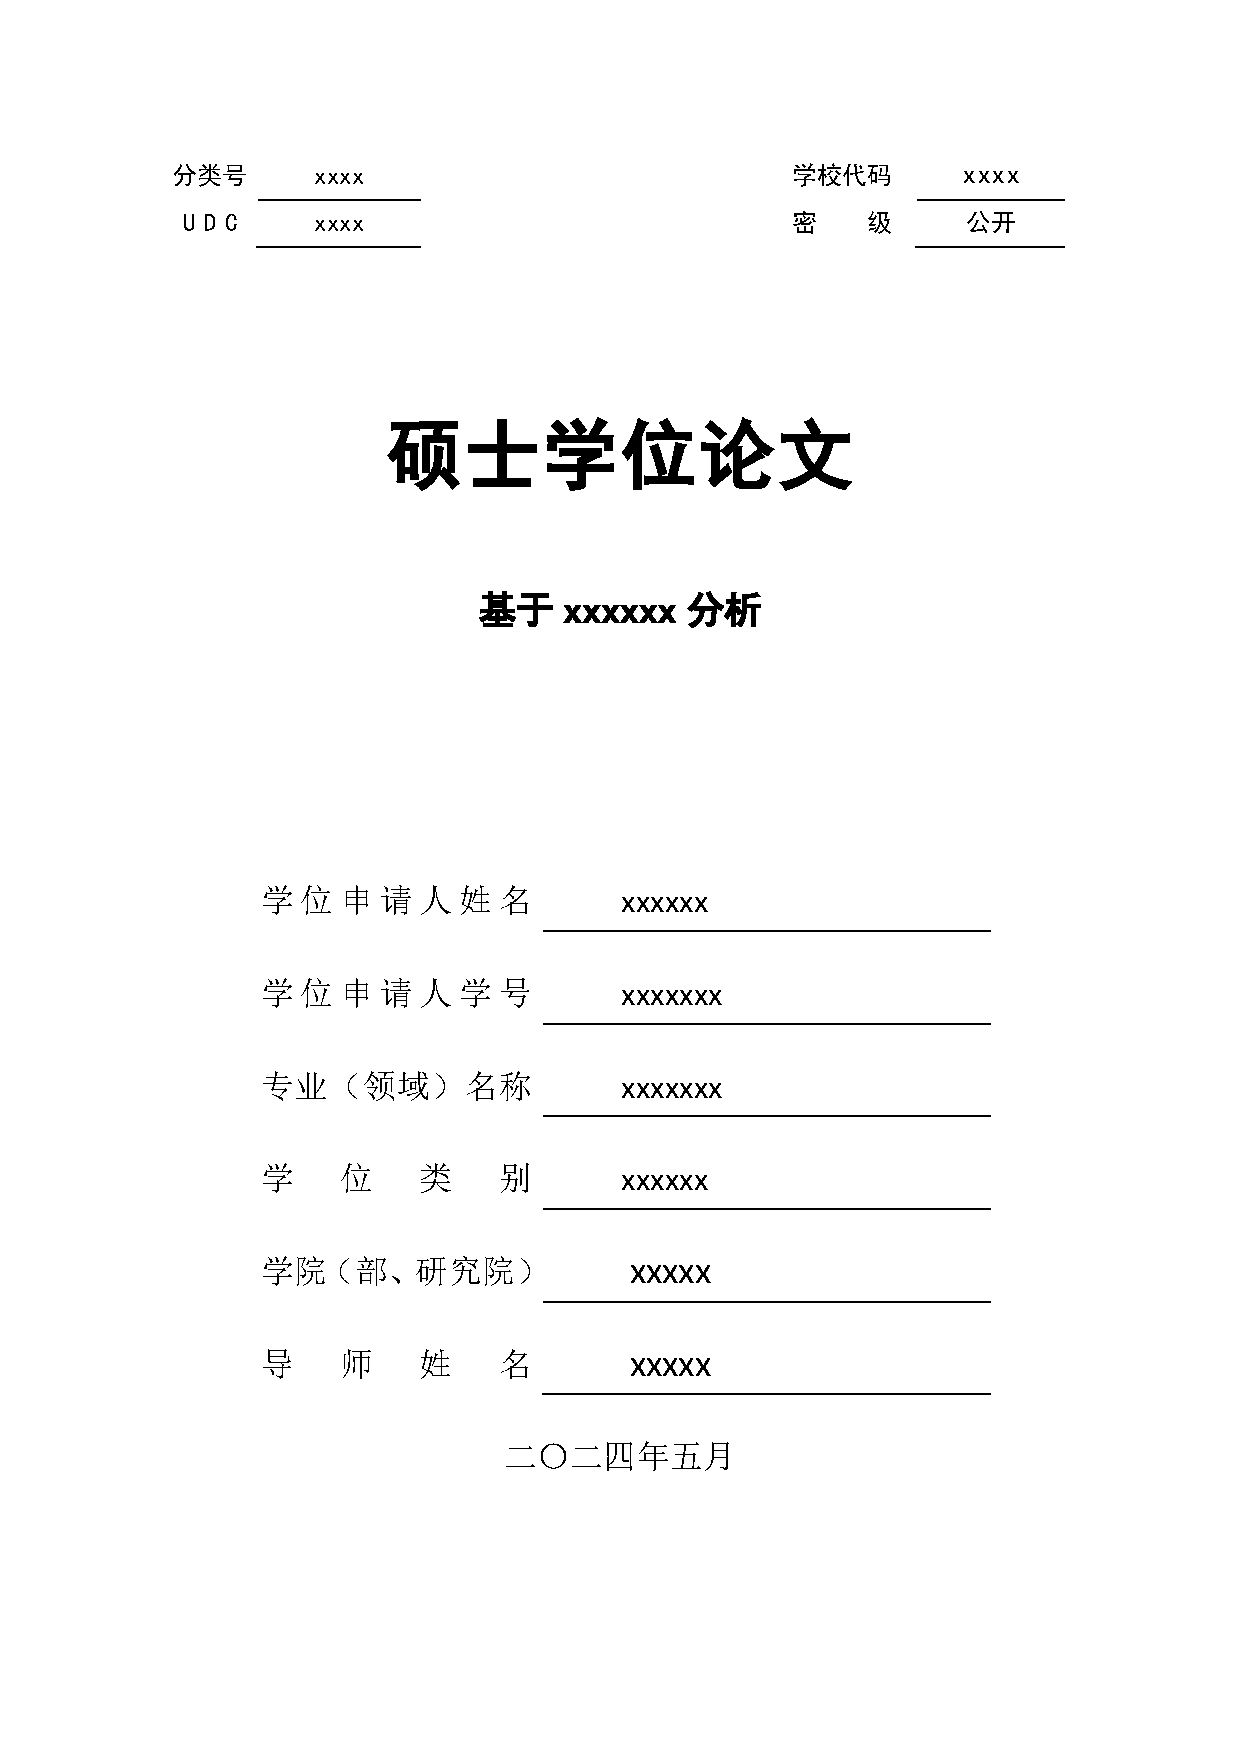
\includepdf[pages=1]{data/cover.pdf}
    \newpage
    \thispagestyle{empty}
    \mbox{}
    \newpage
    \includepdf[pages=2]{data/cover.pdf}
    \newpage
    \thispagestyle{empty}
    \mbox{}
    \newpage
    \cleardoublepage
\else
    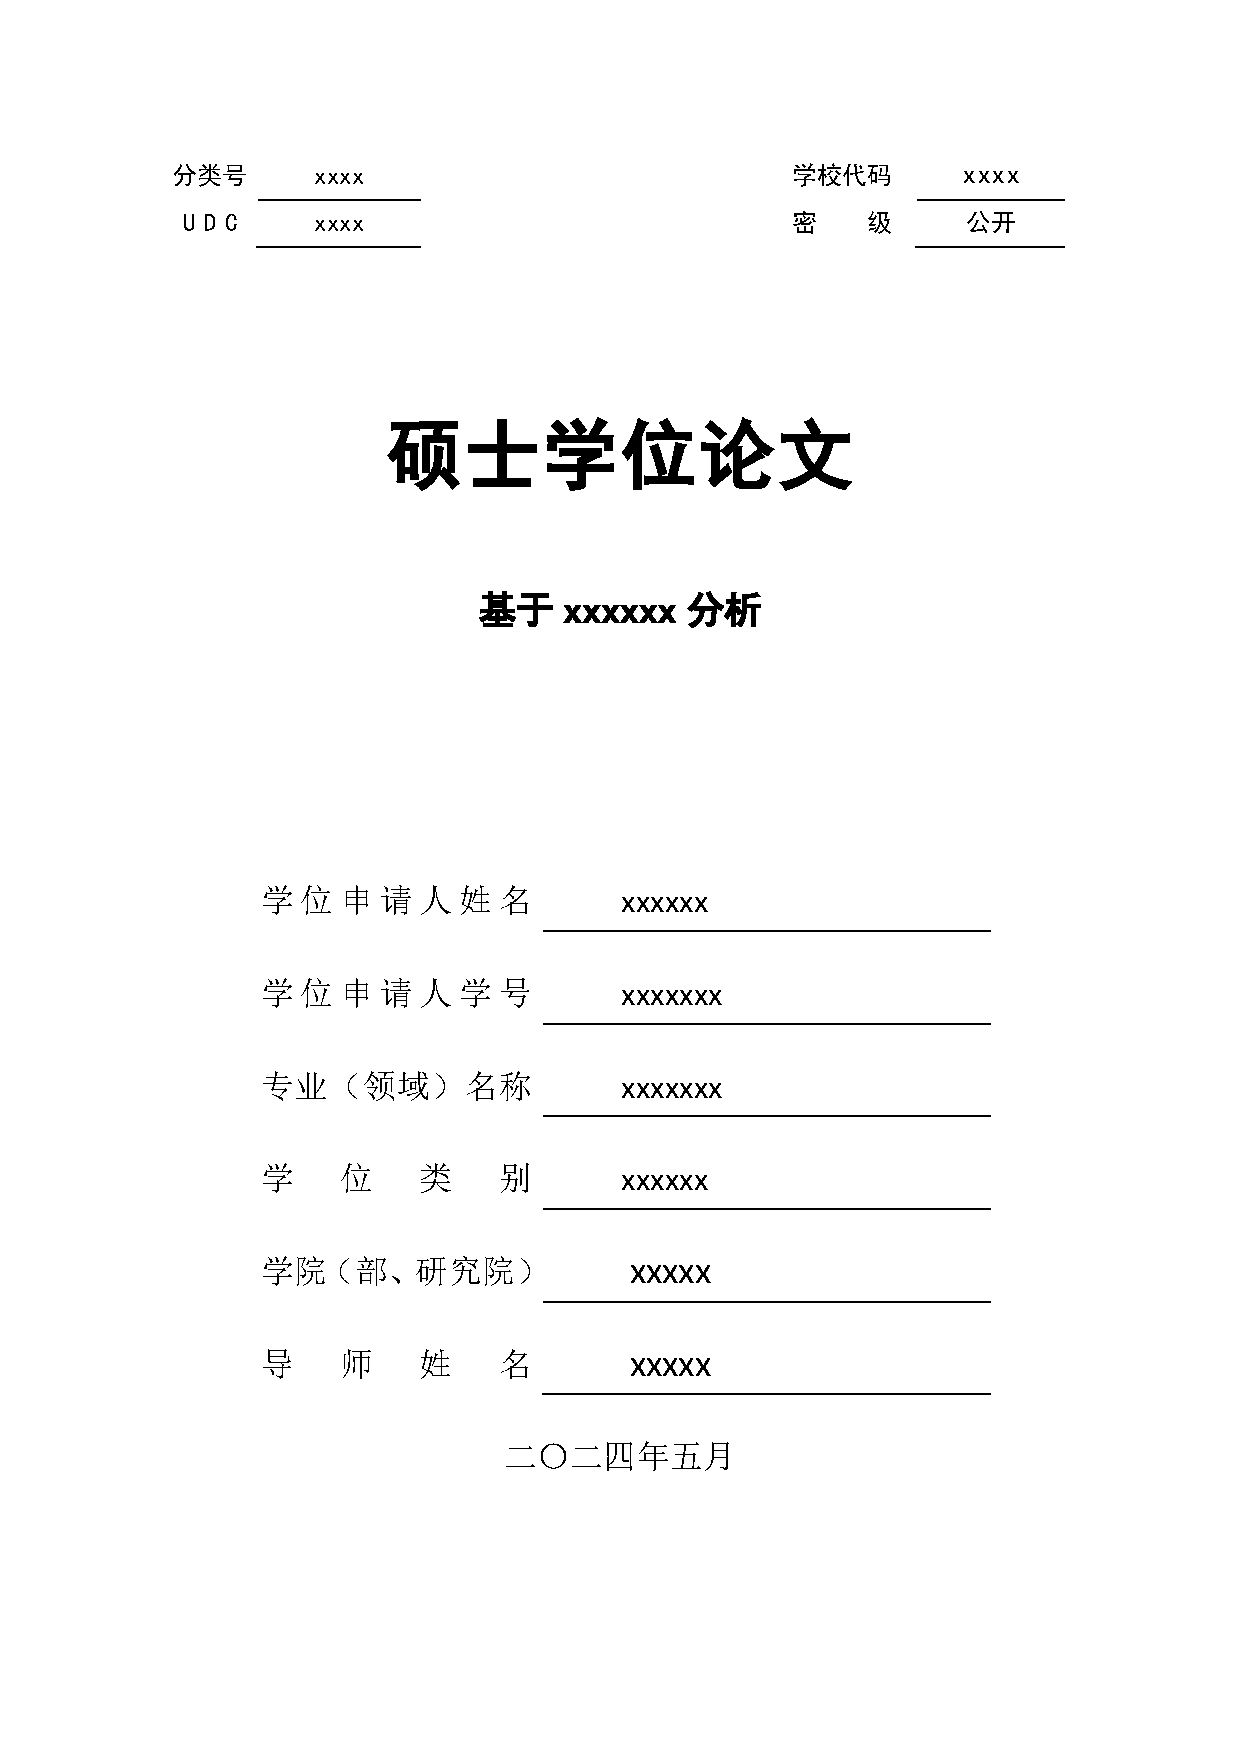
\includepdf[pages=-]{data/cover.pdf}
\fi


% !Mode:: "TeX:UTF-8"

%%% 中文摘要填写部分 %%%
\cnpageheader{基于原神的开放世界冒险游戏加速方法研究} 

\cnabstract{
原神》是一款开放世界的动作角色扮演游戏，玩家至多能够选择四名角色参与战斗，并且在战斗中可以快速切换（冷却时间为1秒）4]。玩家可以通过各种方式增强角色的力量，例如提高角色的等级，改进角色装备的圣遗物和武器5]。除了探索之外，玩家还可以尝试各种挑战以获得奖励。世界中各处散布着头目和挑战，完成后会结予高价值资源，但会消耗随着时间的推移缓慢再生的体力6]。玩家可以通过完成这些挑战以提高冒险等级，进而解锁新的任务、挑战并提升世界等级7]。世界等级是衡量世界上敌人的强大程度以及击败他们所获得奖励的稀有程度的标准8]。

游戏采用开放世界地图，除了正常的步行外，玩家可以通过攀爬、游泳、使用风之翼飞行等移动手段来探索各式各样的遗迹和地形9]10]。玩家在世界中可以与世界中众多设置好的可交互部分互动，如玩家可以在野外遇到可以用于烹饪的木堆，并在其上烹饪，有时碰到的火堆是熄灭的，需要玩家使用火元素手动点燃才可烹饪，已点燃的火堆接触到水元素也会被浇灭11]。一些角色拥有可以改变环境的能力，例如使用冰元素冻结水面来创造一条可以帮助玩家穿越水域地形的冰路4]。世界中存在许多传送锚点，玩家可以借此进行快速旅行，部分传送点也可以恢复和治愈角色，并提供诸如增加玩家耐力等增益12]。食物和矿石可以从开放世界获得，而敌人和宝箱会掉落其他类型的资源，这些资源可以用来增强角色的强度。此外，还有一些被称为“秘境”的特殊战斗空间，也会奖励提升角色和武器强度的材料（例如天赋素材、武器突破素材和圣遗物）。玩家可以通过狩猎动物、采集水果和蔬菜或从商店购买来获取食物13]。烹饪出的食物可以恢复角色的健康或提高各种性能14]。玩家还可以获取可以提炼的矿石，然后用来制造或强化武器15]16]。

每个角色都有元素战技与元素爆发两种技能，元素战技只要招式的冷却时间结束就可以发动，元素爆发则需要累积一定的元素能量才可释放17]18]。角色可以控制七种自然元素冰、草、火、水、风、雷、岩之一19]。这些元素可以以不同的方式相互作用，在战斗中切换角色并执行这些技能可以让这些元素交互发生，发生“元素反应”，打出更高的伤害20]。解决主世界中的谜题可能需要某些元素能力4]。

游戏的多人模式以合作模式进行，允许最多4名玩家可以在主世界或秘境中一起进行游戏21]。玩家匹配可以通过请求与其他玩家联机来完成21]。如果玩家希望与其他玩家一起挑战一个秘境，他们将自动与其他希望解决相同目标的玩家匹配22]。游戏具有跨平台玩法，任何平台的玩家都可以交互23]。

通过完成推进故事的任务，玩家最初可以解锁四个额外的可玩角色（旅行者、安柏、凯亚和丽莎）24]，并且可以通过抽奖机制和游戏内事件获得更多角色或武器25]26]27]。抽奖需要几种高级游戏货币（纠缠之缘和相遇之缘），玩家可以通过游戏内剧情、任务、地图探索等方式或应用内购买获得28]。在抽奖达一定次数后，获得稀有物品的概率会提升，在抽奖获得五星角色/武器后，此概率会重置。29

游戏内亦含有家园系统“尘歌壶”30]，内置集换式卡牌游戏“七圣召唤”31]，以及音乐游戏“千音雅集”32]。



}

{

}

\ckeywords{~~原神；开放世界；冒险游戏}

% 使用makecnabstract生成中文摘要
\makecnabstract
						% 中文摘要
% !Mode:: "TeX:UTF-8"

%%% 英文摘要填写部分 %%%
\cnpageheader{Research on Acceleration Methods for an Open-World Adventure Game Based on Genshin Impact}
\enabstract{
*Genshin Impact* is an open-world action role-playing game in which players can select up to four characters to participate in combat and can quickly switch between them during battle, with a cooldown of one second [4]. Players can enhance characters’ strength in various ways, such as increasing character levels and improving character equipment, including Artifacts and weapons [5]. In addition to exploration, players can attempt various challenges to obtain rewards. Bosses and challenges are scattered throughout the world; completing them grants high-value resources, but consumes Original Resin, a resource that regenerates slowly over time [6]. Players can complete these challenges to increase their Adventure Rank, thereby unlocking new quests and challenges and raising their World Level [7]. World Level is a standard that measures the strength of enemies in the world and the rarity of rewards obtained by defeating them [8].

The game uses an open-world map. In addition to normal walking, players can explore various ruins and terrains through movement methods such as climbing, swimming, and gliding with Wind Gliders [9][10]. Players can interact with many preset interactive elements in the world. For example, players may encounter campfires in the wild that can be used for cooking; sometimes these fires are extinguished and must be manually lit using Pyro before cooking becomes possible. Lit fires can also be extinguished when they come into contact with Hydro [11]. Some characters have abilities that can alter the environment, such as using Cryo to freeze water surfaces and create an ice path that helps players cross bodies of water [4]. Numerous Teleport Waypoints exist throughout the world, allowing players to fast travel. Some teleport points can also restore and heal characters and provide buffs such as increasing the player’s stamina [12]. Food and ore can be obtained from the open world, while enemies and chests drop other types of resources that can be used to strengthen characters. In addition, special combat spaces known as “Domains” reward materials used to improve characters and weapons, such as Talent Materials, Weapon Ascension Materials, and Artifacts. Players can obtain food by hunting animals, gathering fruits and vegetables, or purchasing it from shops [13]. Cooked food can restore characters’ health or improve various attributes [14]. Players can also obtain ores that can be refined and then used to craft or enhance weapons [15][16].

Each character has two types of abilities: an Elemental Skill and an Elemental Burst. An Elemental Skill can be used once its cooldown ends, while an Elemental Burst requires a certain amount of Elemental Energy before it can be released [17][18]. Characters can control one of seven natural elements: Cryo, Dendro, Pyro, Hydro, Anemo, Electro, and Geo [19]. These elements can interact with one another in different ways. By switching characters during combat and using these abilities, players can trigger interactions between elements, known as “Elemental Reactions,” to deal higher damage [20]. Solving puzzles in the overworld may also require certain elemental abilities [4].

The game’s multiplayer mode is cooperative, allowing up to four players to play together in the overworld or in Domains [21]. Players can match with others by requesting to join another player’s world [21]. If players wish to challenge a Domain with others, they are automatically matched with other players who wish to complete the same objective [22]. The game supports cross-platform play, allowing players on different platforms to interact with one another [23].

}

\enkeywords{Processing-in-Memory; Graph Neural Networks; Graph-based Retrieval-Augmented Generation}
 
\enpageheader{Research on Acceleration Methods for an Open-World Adventure Game Based on Genshin Impact}

\makeenabstract
						% 英文摘要

\pagestyle{empty}		% modified by Jon: 去掉页眉页脚
% 目录
\renewcommand{\contentsname}{\sanhao\hei\bfseries\hspace*{\fill}\text{目}\quad \text{录}\hspace*{\fill}}    % 设置“目录”二字的格式

\renewcommand{\listfigurename}{\sanhao\hei\bfseries\hspace*{\fill}\text{图}\quad \text{索}\quad \text{引}\hspace*{\fill}}    % 设置“目录”二字的格式

\renewcommand{\listtablename}{\sanhao\hei\bfseries\hspace*{\fill}\text{表}\quad \text{索}\quad \text{引}\hspace*{\fill}}    % 设置“目录”二字的格式

\renewcommand{\listalgorithmname}{\sanhao\hei\bfseries\hspace*{\fill}\text{算}\quad \text{法}\quad \text{索}\quad \text{引}\hspace*{\fill}}    % 设置“目录”二字的格式

\newcommand{\myhl}[1]{\colorbox{yellow}{#1}} % 自定义高亮命令

\newcolumntype{C}[1]{>{\centering\arraybackslash}p{#1}}

\tableofcontents                % 中文目录
\cleardoublepage

\pagestyle{empty}
\listoffigures
\thispagestyle{empty}
\ifprintstyle
    \cleardoublepage
\fi


\pagestyle{empty}
\listoftables
\thispagestyle{empty}
\ifprintstyle
    \cleardoublepage
\fi

\pagestyle{empty}
\listofalgorithms
\thispagestyle{empty}
\ifprintstyle
    \cleardoublepage
\fi

% 正文部分
\defaultfont
\pagestyle{plain}
\mainmatter\sloppy\raggedbottom
%\renewcommand{\ALC@linenosize}{\xiaosi}
\renewcommand\arraystretch{1.5}
\renewcommand{\algorithmicrequire}{\textbf{输入:}}
\renewcommand{\algorithmicensure}{\textbf{输出:}}
\setlength{\intextsep}{2pt}
\setlength{\abovecaptionskip}{2pt}
\setlength{\belowcaptionskip}{2pt}

% 内容比较多的时候，编译速度较慢，可以将不同章节放在不同文件中，注释掉其他章节，只编译正在撰写的章节，以提升编译速度

% !Mode:: "TeX:UTF-8"
\chapter{绪论}
\label{chapter:intro}
\cnpageheader{第一章~~~~绪论}

\section{研究背景}
我是研究背景
我是研究背景
我是研究背景


\section{国内外研究现状}
\subsection{XXX相关研究}




\section{本文的研究内容与创新点}

本文围绕


综上， 

第一， 。

第二， 


\section{本文的组织结构}



本论文总共分为五个章节，顺序

% !Mode:: "TeX:UTF-8"
\chapter{背景知识}
\label{chapter:background}
\cnpageheader{第二章~~~~背景知识}


本章旨在系统阐述本研究涉及的关键背景知识与技术基础，为后续研究工作提供理论支撑。
xxx oiuwhiudsasidgbasgbdsadbshad
sadsa sad as




\section{图神经网络}

图神经网络（Graph Neural Networks, GNNs）是一类专门用于处理图结构数据的深度学习模型，并被广泛用于处理图的特征表示~\cite{kipf2016semi}。
中，第$k$层的卷积运算可以总结为以下公式。
\begin{align} 
c_v^k &=\text{\textbf{Combine}} \left(h_v^{k-1} \right) \\
h_v^k &=\text{\textbf{Aggregate}} \left(c_u^k|u\in N(v) \cup \{v\} \right) 
\end{align}
最终经过跨多层的迭代计算，输出将包含顶点的原始特征、邻居特征以及输入图的结构信息。



\section{本章小结}
本章围绕后续研
% !Mode:: "TeX:UTF-8"


\chapter{XXXX架构}
\label{chapter:iter}
\cnpageheader{第三章~~XXXX架构}


\section{研究动机}


\section{本章小结}
本章针对
% !Mode:: "TeX:UTF-8"


\chapter{XXXX架构22}
\label{chapter:iter}
\cnpageheader{第四章~~XXXX架构}


\section{研究动机}


\section{本章小结}
本章针对
% !Mode:: "TeX:UTF-8"
\label{chapter:conclusionee}
\chapter{总结与展望}
\cnpageheader{第五章~~~~总结与展望}

\section{总结}
总结总结总结总结总结




\section{展望}
展望展望展望展望


\defaultfont
\bibliographystyle{gbt7714-numerical}
\phantomsection
\cnpageheader{参考文献}
\addcontentsline{toc}{chapter}{参考文献}          
\bibliography{references}	
\renewcommand\thefigure{A.\arabic{figure}}			% 将附录中的图像的id的章节num设置为A

% !Mode:: "TeX:UTF-8"
\cnpageheader{致谢}

\begin{theacknowledgements}
这是致谢，谢谢你也谢谢我 thank you
\end{theacknowledgements}

						% 致谢

% !Mode:: "TeX:UTF-8"
\cnpageheader{攻读硕士学位期间的研究成果}

\newenvironment{thepublications}{\wuhao\song}

\addcontentsline{toc}{chapter}{攻读硕士学位期间的研究成果}%添加到目录中
\chapter*{\centering\sanhao\heiti\bfseries\textbf{攻读硕士学位期间的研究成果}}
\titlespacing{\chapter}{0pt}{24pt}{18pt}

\begin{thepublications}

\setlength{\parindent}{0em}

\textbf{一、学术论文}

\begin{publist}
    \item \textbf{Yuanshen}, XXX, YYY, ``Wo ai wan yuan shen", in YUANSHEN Conference (YC), 2025, pp. 1-7.（\textbf{YS-A类会议}，\textbf{第一作者}，已发表）
\end{publist}

~

\textbf{二、发明专利}
  
\begin{publist}
    \item \textbf{原神}; 原神2; 原神3, ZL202223232323, 一种原神存储方法、装置及电子设备.（已授权，\textbf{第一发明人}）
\end{publist}

\vfill
\hangafter=1\hangindent=2em\noindent
\setlength{\parindent}{2em}
\end{thepublications}

							% 研究成果

% 针对附录重新定义目录格式，去掉页码和前面的点
\titlecontents{chapter}
    [0em] % 左边距
    {\song\fontsize{12pt}{20pt}\selectfont} % 前缀格式
    {} % 章节号
    {} % 无章节号时的处理
    {\titlerule*[5pt]{}} % 页码前的填充
\titlecontents{subsection}
    [2em]
    {\song\fontsize{12pt}{20pt}\selectfont} %
    {\thecontentslabel\quad}{} %
    {\hspace{.25em}\titlerule*[5pt]{}}
    
% \addcontentsline{toc}{chapter}{附：指导教师对研究生学位论文的学术评语}
% \includepdf[pages=-]{data/comment.pdf}

% \addcontentsline{toc}{subsection}{答辩委员会决议书}
% \includepdf[pages=-]{data/decision.pdf}

\clearpage
\end{document}                                   
